%Version 3.1 December 2024
% See section 11 of the User Manual for version history
%
%%%%%%%%%%%%%%%%%%%%%%%%%%%%%%%%%%%%%%%%%%%%%%%%%%%%%%%%%%%%%%%%%%%%%%
%%                                                                 %%
%% Please do not use \input{...} to include other tex files.       %%
%% Submit your LaTeX manuscript as one .tex document.              %%
%%                                                                 %%
%% All additional figures and files should be attached             %%
%% separately and not embedded in the \TeX\ document itself.       %%
%%                                                                 %%
%%%%%%%%%%%%%%%%%%%%%%%%%%%%%%%%%%%%%%%%%%%%%%%%%%%%%%%%%%%%%%%%%%%%%

%%\documentclass[referee,sn-basic]{sn-jnl}% referee option is meant for double line spacing

%%=======================================================%%
%% to print line numbers in the margin use lineno option %%
%%=======================================================%%

%%\documentclass[lineno,pdflatex,sn-basic]{sn-jnl}% Basic Springer Nature Reference Style/Chemistry Reference Style

%%=========================================================================================%%
%% the documentclass is set to pdflatex as default. You can delete it if not appropriate.  %%
%%=========================================================================================%%

% \documentclass[sn-basic]{sn-jnl}% Basic Springer Nature Reference Style/Chemistry Reference Style

%%Note: the following reference styles support Namedate and Numbered referencing. By default the style follows the most common style. To switch between the options you can add or remove “Numbered” in the optional parenthesis. 
%%The option is available for: sn-basic.bst, sn-chicago.bst%  
 
%%\documentclass[pdflatex,sn-nature]{sn-jnl}% Style for submissions to Nature Portfolio journals
% \documentclass[pdflatex,sn-basic]{sn-jnl}% Basic Springer Nature Reference Style/Chemistry Reference Style
\documentclass[pdflatex,sn-mathphys-num]{sn-jnl}% Math and Physical Sciences Numbered Reference Style
% Source-review markers are no-op by default and are not printed.
\providecommand{\reviewermap}[3]{}
%%\documentclass[pdflatex,sn-mathphys-ay]{sn-jnl}% Math and Physical Sciences Author Year Reference Style
%%\documentclass[pdflatex,sn-aps]{sn-jnl}% American Physical Society (APS) Reference Style
%%\documentclass[pdflatex,sn-vancouver-num]{sn-jnl}% Vancouver Numbered Reference Style
%%\documentclass[pdflatex,sn-vancouver-ay]{sn-jnl}% Vancouver Author Year Reference Style
%%\documentclass[pdflatex,sn-apa]{sn-jnl}% APA Reference Style
%%\documentclass[pdflatex,sn-chicago]{sn-jnl}% Chicago-based Humanities Reference Style

%%%% Standard Packages
%%<additional latex packages if required can be included here>

\usepackage{graphicx}%
\usepackage{multirow}%
\usepackage{amsmath,amssymb,amsfonts}%
\usepackage{amsthm}%
\usepackage{mathrsfs}%
\usepackage[title]{appendix}%
\usepackage{xcolor}%
\usepackage{textcomp}%
\usepackage{manyfoot}%
\usepackage{booktabs}%
\usepackage{algorithm}%
\usepackage{algorithmicx}%
\usepackage{algpseudocode}%
\usepackage{listings}%

% User defined
%%%%Userd-added package
\usepackage[version=3]{mhchem}
\usepackage{subcaption}
\usepackage{graphicx}
\usepackage{float}
\usepackage{multirow}
\usepackage{array}
\usepackage{amsmath}
\usepackage{booktabs}
\usepackage{amsmath}
\usepackage{amssymb}
\usepackage{xcolor}

\usepackage[utf8]{inputenc} % allow utf-8 input
\usepackage{hyperref}       % hyperlinks
\usepackage{url}            % simple URL typesetting
\usepackage{amsfonts}       % blackboard math symbols
\usepackage{nicefrac}       % compact symbols for 1/2, etc.
\usepackage{microtype}      % microtypography

\usepackage{xr}
\externaldocument{sn-article-SI}
%%%%
\newcommand{\pc}[1]{{\color{purple}[Paulette: #1]}}
\newcommand{\yi}[1]{{\color{teal}[Yi: #1]}}
%%%%%=============================================================================%%%%
%%%%  Remarks: This template is provided to aid authors with the preparation
%%%%  of original research articles intended for submission to journals published 
%%%%  by Springer Nature. The guidance has been prepared in partnership with 
%%%%  production teams to conform to Springer Nature technical requirements. 
%%%%  Editorial and presentation requirements differ among journal portfolios and 
%%%%  research disciplines. You may find sections in this template are irrelevant 
%%%%  to your work and are empowered to omit any such section if allowed by the 
%%%%  journal you intend to submit to. The submission guidelines and policies 
%%%%  of the journal take precedence. A detailed User Manual is available in the 
%%%%  template package for technical guidance.
%%%%%=============================================================================%%%%

%% as per the requirement new theorem styles can be included as shown below
\theoremstyle{thmstyleone}%
\newtheorem{theorem}{Theorem}%  meant for continuous numbers
%%\newtheorem{theorem}{Theorem}[section]% meant for sectionwise numbers
%% optional argument [theorem] produces theorem numbering sequence instead of independent numbers for Proposition
\newtheorem{proposition}[theorem]{Proposition}% 
%%\newtheorem{proposition}{Proposition}% to get separate numbers for theorem and proposition etc.

\theoremstyle{thmstyletwo}%
\newtheorem{example}{Example}%
\newtheorem{remark}{Remark}%

\theoremstyle{thmstylethree}%
\newtheorem{definition}{Definition}%

\raggedbottom
%%\unnumbered% uncomment this for unnumbered level heads

\begin{document}

\title[Article Title]{Migration as a Probe: A Generalizable Benchmark Framework for Specialist vs. Generalist Machine-Learned Force Fields}
%% change to a new title
\title[Article Title]{Non-Equilibrium Probes Reveal the Limits of Specialist and Foundation Machine-Learned Force Fields}
%%=============================================================%%
%% GivenName	-> \fnm{Joergen W.}
%% Particle	-> \spfx{van der} -> surname prefix
%% FamilyName	-> \sur{Ploeg}
%% Suffix	-> \sfx{IV}
%% \author*[1,2]{\fnm{Joergen W.} \spfx{van der} \sur{Ploeg} 
%%  \sfx{IV}}\email{iauthor@gmail.com}
%%=============================================================%%

\author[1]{\fnm{Yi} \sur{Cao}}\email{ycao73@jh.edu}

\author[1]{\fnm{Peter} \sur{Mastracco}}\email{pmastra2@jh.edu}
% \author[1]{\fnm{Victor} \sur{Wu}}\email{vwu16@jhu.edu}
% % \equalcont{These authors contributed equally to this work.}

\author*[1]{\fnm{Paulette} \sur{Clancy}}\email{pclancy3@jhu.edu}
% \equalcont{These authors contributed equally to this work.}

\affil[1]{\orgdiv{Department of Chemical and Biomolecular Engineering}, \orgname{ Johns Hopkins University}, \orgaddress{\street{3400 N. Charles Street}, \city{Baltimore}, \postcode{21218}, \state{Maryland}, \country{USA}}}

%%==================================%%
%% Sample for unstructured abstract %%
%%==================================%%

% \abstract{The abstract serves both as a general introduction to the topic and as a brief, non-technical summary of the main results and their implications. Authors are advised to check the author instructions for the journal they are submitting to for word limits and if structural elements like subheadings, citations, or equations are permitted.}

\abstract{Machine-learned force fields (MLFFs), particularly pre-trained foundation models, are extending \textit{ab initio}-accurate molecular dynamics to realistic length and time scales. Yet a fundamental question remains: for new materials, should one rely on specialist models, fine-tuned foundation models, or a hybrid approach? The trade-offs in data efficiency, robustness, and non-equilibrium fidelity—and how different training paradigms encode physical information—remain poorly understood.

Here, we introduce a unified benchmarking framework based on non-equilibrium configuration probes spanning interpolation and extrapolation regimes. Migration pathways computed via Nudged Elastic Band calculations serve as the primary diagnostic, complemented by equilibrium and mechanical tests. Using Cr-doped \ce{Sb2Te3} as a representative 2D material, we evaluate multiple training strategies within the MACE architecture.

While all models reproduce equilibrium structures, they diverge sharply for non-equilibrium processes. Fine-tuned models improve kinetic accuracy but degrade long-range mechanical response, whereas zero-shot foundation models exhibit overly smoothed potentials and specialist models fail to extrapolate to high-energy transitions. Latent-space analysis reveals fundamentally distinct learned representations across training paradigms, explaining why equilibrium metrics alone are insufficient.

\reviewermap{REV-A4}{done-local}{Scope generalizable-standard language to a candidate framework demonstrated on Cr-doped Sb2Te3.}
This work demonstrates migration-based non-equilibrium probes as a data-efficient candidate framework for MLFF evaluation, developed and tested on one representative material system, and provides practical guidance for robust MLFF development.
}
%%================================%%
%% Sample for structured abstract %%
%%================================%%

% \abstract{\textbf{Purpose:} The abstract serves both as a general introduction to the topic and as a brief, non-technical summary of the main results and their implications. The abstract must not include subheadings (unless expressly permitted in the journal's Instructions to Authors), equations or citations. As a guide the abstract should not exceed 200 words. Most journals do not set a hard limit however authors are advised to check the author instructions for the journal they are submitting to.
% 
% \textbf{Methods:} The abstract serves both as a general introduction to the topic and as a brief, non-technical summary of the main results and their implications. The abstract must not include subheadings (unless expressly permitted in the journal's Instructions to Authors), equations or citations. As a guide the abstract should not exceed 200 words. Most journals do not set a hard limit however authors are advised to check the author instructions for the journal they are submitting to.
% 
% \textbf{Results:} The abstract serves both as a general introduction to the topic and as a brief, non-technical summary of the main results and their implications. The abstract must not include subheadings (unless expressly permitted in the journal's Instructions to Authors), equations or citations. As a guide the abstract should not exceed 200 words. Most journals do not set a hard limit however authors are advised to check the author instructions for the journal they are submitting to.
% 
% \textbf{Conclusion:} The abstract serves both as a general introduction to the topic and as a brief, non-technical summary of the main results and their implications. The abstract must not include subheadings (unless expressly permitted in the journal's Instructions to Authors), equations or citations. As a guide the abstract should not exceed 200 words. Most journals do not set a hard limit however authors are advised to check the author instructions for the journal they are submitting to.}

\keywords{Machine-learned force fields (MLFFs), foundation models, fine-tuning, defect migration pathways, 2D materials}

%%\pacs[JEL Classification]{D8, H51}

%%\pacs[MSC Classification]{35A01, 65L10, 65L12, 65L20, 65L70}

\maketitle

\section{Introduction}

Machine-Learned Force Fields (MLFFs)~\citep{unke_machine_2021, ssmith_ani-1_2017, chen_accurate_2017, batatia_mace_nodate,vandermause_active_2022, batzner_e3-equivariant_2022, bartok_gaussian_2010, friederich2021machine, zeng_deepmd-kit_2023, wines_chips-ff_2025, musaelian_learning_2023, chen_universal_2022, lindsey2017chimes,  xie2018crystal} have emerged as a transformative solution to the dilemma of accuracy-versus-cost in molecular simulation. The recent development of large-scale, pre-trained ``foundation models,'' such as CHGNet,~\citep{deng_chgnet_2023} MEGNet,~\citep{chen_graph_2019} M3GNet,~\citep{chen_universal_2022} MACE-MP,~\citep{batatia_mace_nodate} MatterSim,~\citep{yang_mattersim_2024} and UMA,~\citep{wood_uma_2025} marks a paradigm shift to try to resolve this dilemma.~\citep{merchant_scaling_2023}.This shift presents researchers with a critical question: For a specific system, is it more effective to invest significant resources to build a robust \textit{specialist} model from scratch,~\citep{zhang_deep_2018, smith_approaching_2017, chmiela_sgdml_2017} or to adapt a \textit{generalist} foundation model through fine-tuning? While generic benchmarks like Matbench,~\citep{dunn_benchmarking_2020} JARVIS-Leaderboard,~\citep{choudhary2024jarvis} and LeMat-GenBench,~\citep{betala2025lemat} validate their broad utility, their reliability for specific, high-fidelity applications remains an open question.~\citep{friederich_machine-learned_2021, deringer_machine_2019, jacobs2025practical}  A valid concern is that these models may fail to capture nuanced interactions governing critical processes that shape the materials and their processing. ~\citep{schran_machine_2020, kapil_assessment_2022, grisafi_transferable_2018, liu2023discrepancies} Fine-tuning is a promising solution, but naïve strategies can lead to \textit{``catastrophic forgetting''}, where general knowledge is erased. Key questions of data efficiency,~\citep{janet_designing_2019, lookman_active_2019} stability,~\citep{zuo_performance_2020, jinnouchi_phase_2020} and transferability~\citep{zeni_data_2021, vandermause_on--fly_2020} for non-equilibrium processes remain largely unsolved. ~\citep{bernstein_quantifying_2019, zhang_active_2019, he2018statistical}



To build a rigorous benchmark that addresses the specialist-generalist dilemma, we must answer three fundamental questions: \textit{What} defines a good model beyond simple accuracy metrics? \textit{How} do different training strategies—from scratch, zero-shot, or fine-tuning, shape what the model learns? \textit{Why} do certain models succeed or fail, and can we open the ``black box'' to understand root causes? Current evaluation approaches rely heavily on equilibrium properties and traditional numerical metrics like RMSE. But these approaches may not capture the stringent requirements needed for dynamic processes that are critical to materials' functionality.~\citep{fu2022forces, mannan2025evaluating} When an MLFF-driven simulation fails, the underlying cause is often treated as a `black box,'' with the default response being indiscriminate addition of more data, a brute-force approach that wastes resources.

%%%%% updated for broader tone discussing about the non-equilibrium data's importance 
We propose that overcoming this limitation requires evaluation strategies that probe a model’s behavior under controlled non-equilibrium lattice distortions rather than relying solely on equilibrium structures. In this spirit, migration-pathway methods based on the Nudged Elastic Band (NEB) algorithm~\citep{miskin2025low, ruttinger_protocol_2022, cao2025migration, he2017origin,bheemaguli2026mlipBarriers} offer a broadly applicable way to generate structured, physically motivated perturbations that expose how a force field behaves when pushed beyond small displacements. Although originally designed to characterize transition paths, these trajectories naturally span intermediate configurations that are far more discriminating than static tests, revealing stability and generalization gaps that conventional metrics tend to obscure. This perspective motivates the benchmarking framework developed in this work, which uses such non-equilibrium configuration sequences to sharpen model comparisons and to uncover the conditions under which different training strategies succeed or fail.

To demonstrate and validate this benchmarking framework, we employ doped two-dimensional (2D) van der Waals (vdW) materials as an ideal test bed. The discovery and design of novel 2D vdW materials~\citep{novoselov_2d_2016, manzeli_2d_2017, akinwande2017review, guo_stacking_2021, liu_roadmap_2024} continues to drive innovation in spintronics,~\citep{he_topological_2022} quantum devices,~\citep{qian_van_2024, song_electron_2018, nayak_microsoft_2025} and energy technologies.~\citep{jin_flexible_2019,gautam_creation_2024} A particularly powerful strategy for tuning the properties of these layered materials involves doping, the insertion of ``foreign'' atoms between vdW layers.~\citep{novoselov_2d_2016, whittingham_lithium_2004} This approach has enabled remarkable advances in materials design, ranging from lithium-ion batteries~\citep{winter_insertion_1998, hu_lithium_2024} to the engineering of magnetic semiconductors~\citep{gibertini_magnetic_2019} and quantum anomalous Hall systems.~\citep{tokura_magnetic_2019} Crucially, their layered structure offers distinct environments for atomic motion, making them an excellent probe for testing MLFF capabilities across different chemical contexts within a single system.

Among 2D materials, topological insulators such as antimony telluride (\ce{Sb2Te3})~\citep{zhang_topological_2009, guo_roadmap_2015} represent an especially promising class for doping studies. The doping of transition metals has proven effective across multiple topological systems: Iron in \ce{Bi2Se3} creates ferromagnetic order~\citep{checkelsky_trajectory_2014, kulbachinskii_thermoelectric_2012, haazen_ferromagnetism_2012}. Manganese in \ce{Bi2Te3} enables tunable magnetic properties.~\citep{klimovskikh_tunable_2020, fu_electronic_2021} And vanadium in \ce{Sb2Te3} modifies its electronic structure.~\citep{sun_sb2te3_2023, zhang_quantum_2021} The doping of chromium (Cr) into \ce{Sb2Te3}, the focus of this work, offers a compelling route to engineer its magnetic and topological properties for spintronic applications.~\citep{cortie_creating_2020,han_effect_2013,de_a_deus_magnetic_2021} Predicting the stability and dynamics of these complex systems is essential for guiding experimental synthesis, a task for which large-scale Molecular Dynamics (MD) simulations are extremely powerful~\citep{Zhang2023TuningStudy,thompson_lammps_2022} provided that a suitably representative force field is available. However, the atomic-scale processes governing functionality, including dopant migration and thermal stability, occur on time- and length- scales far beyond the reach of first-principles methods like density functional theory (DFT).~\citep{kohn_self-consistent_1965, perdew_generalized_1996, sohier_density_2017,choudhary_high-throughput_2017}

This work addresses these gaps by presenting a systematic benchmark of bespoke training and fine-tuning strategies for the case study of Cr-doped \ce{Sb2Te3} using the MACE architecture (Fig.~\ref{fig:conceptual_diagram}). By combining latent-space analysis with migration-based probes, we move beyond traditional accuracy metrics to evaluate the dynamic stability and kinetic predictions of each model. Our study aims to serve as both a practical guide for selecting MLFF training strategies and a diagnostic framework for designing more data-efficient learning loops. 
\reviewermap{REV-A7}{done-local}{Add nearest-neighbor literature and state the delta relative to the earlier arXiv/workshop report.}
This manuscript extends our earlier report~\citep{cao2025migration} by adding a unified fixed-path and self-consistent NEB analysis, interlayer sliding tests, representation diagnostics, and a data provenance workflow. It therefore treats migration pathways not only as an application result, but also as a structured benchmark distribution for testing model behavior under task-relevant distribution shift.

To this end, we address the following key questions:
\begin{enumerate}
\item How do bespoke MLFFs trained from scratch compare against large pre-trained foundation models in terms of accuracy, stability, and data efficiency for molecular simulation? What are the performance and stability trade-offs of different fine-tuning strategies?
\reviewermap{REV-A4}{done-local}{Frame generalizability as an open question rather than a completed claim.}
\item Can non-equilibrium probes generated from methods, such as NEB, provide an efficient benchmark for specialist versus generalist models, and what additional cross-system evidence is needed before such probes can be considered general across materials and architectures?
\item Can latent-space analysis reveal failure signatures to guide data acquisition?
\end{enumerate}

\begin{figure}[htbp]
    \centering
    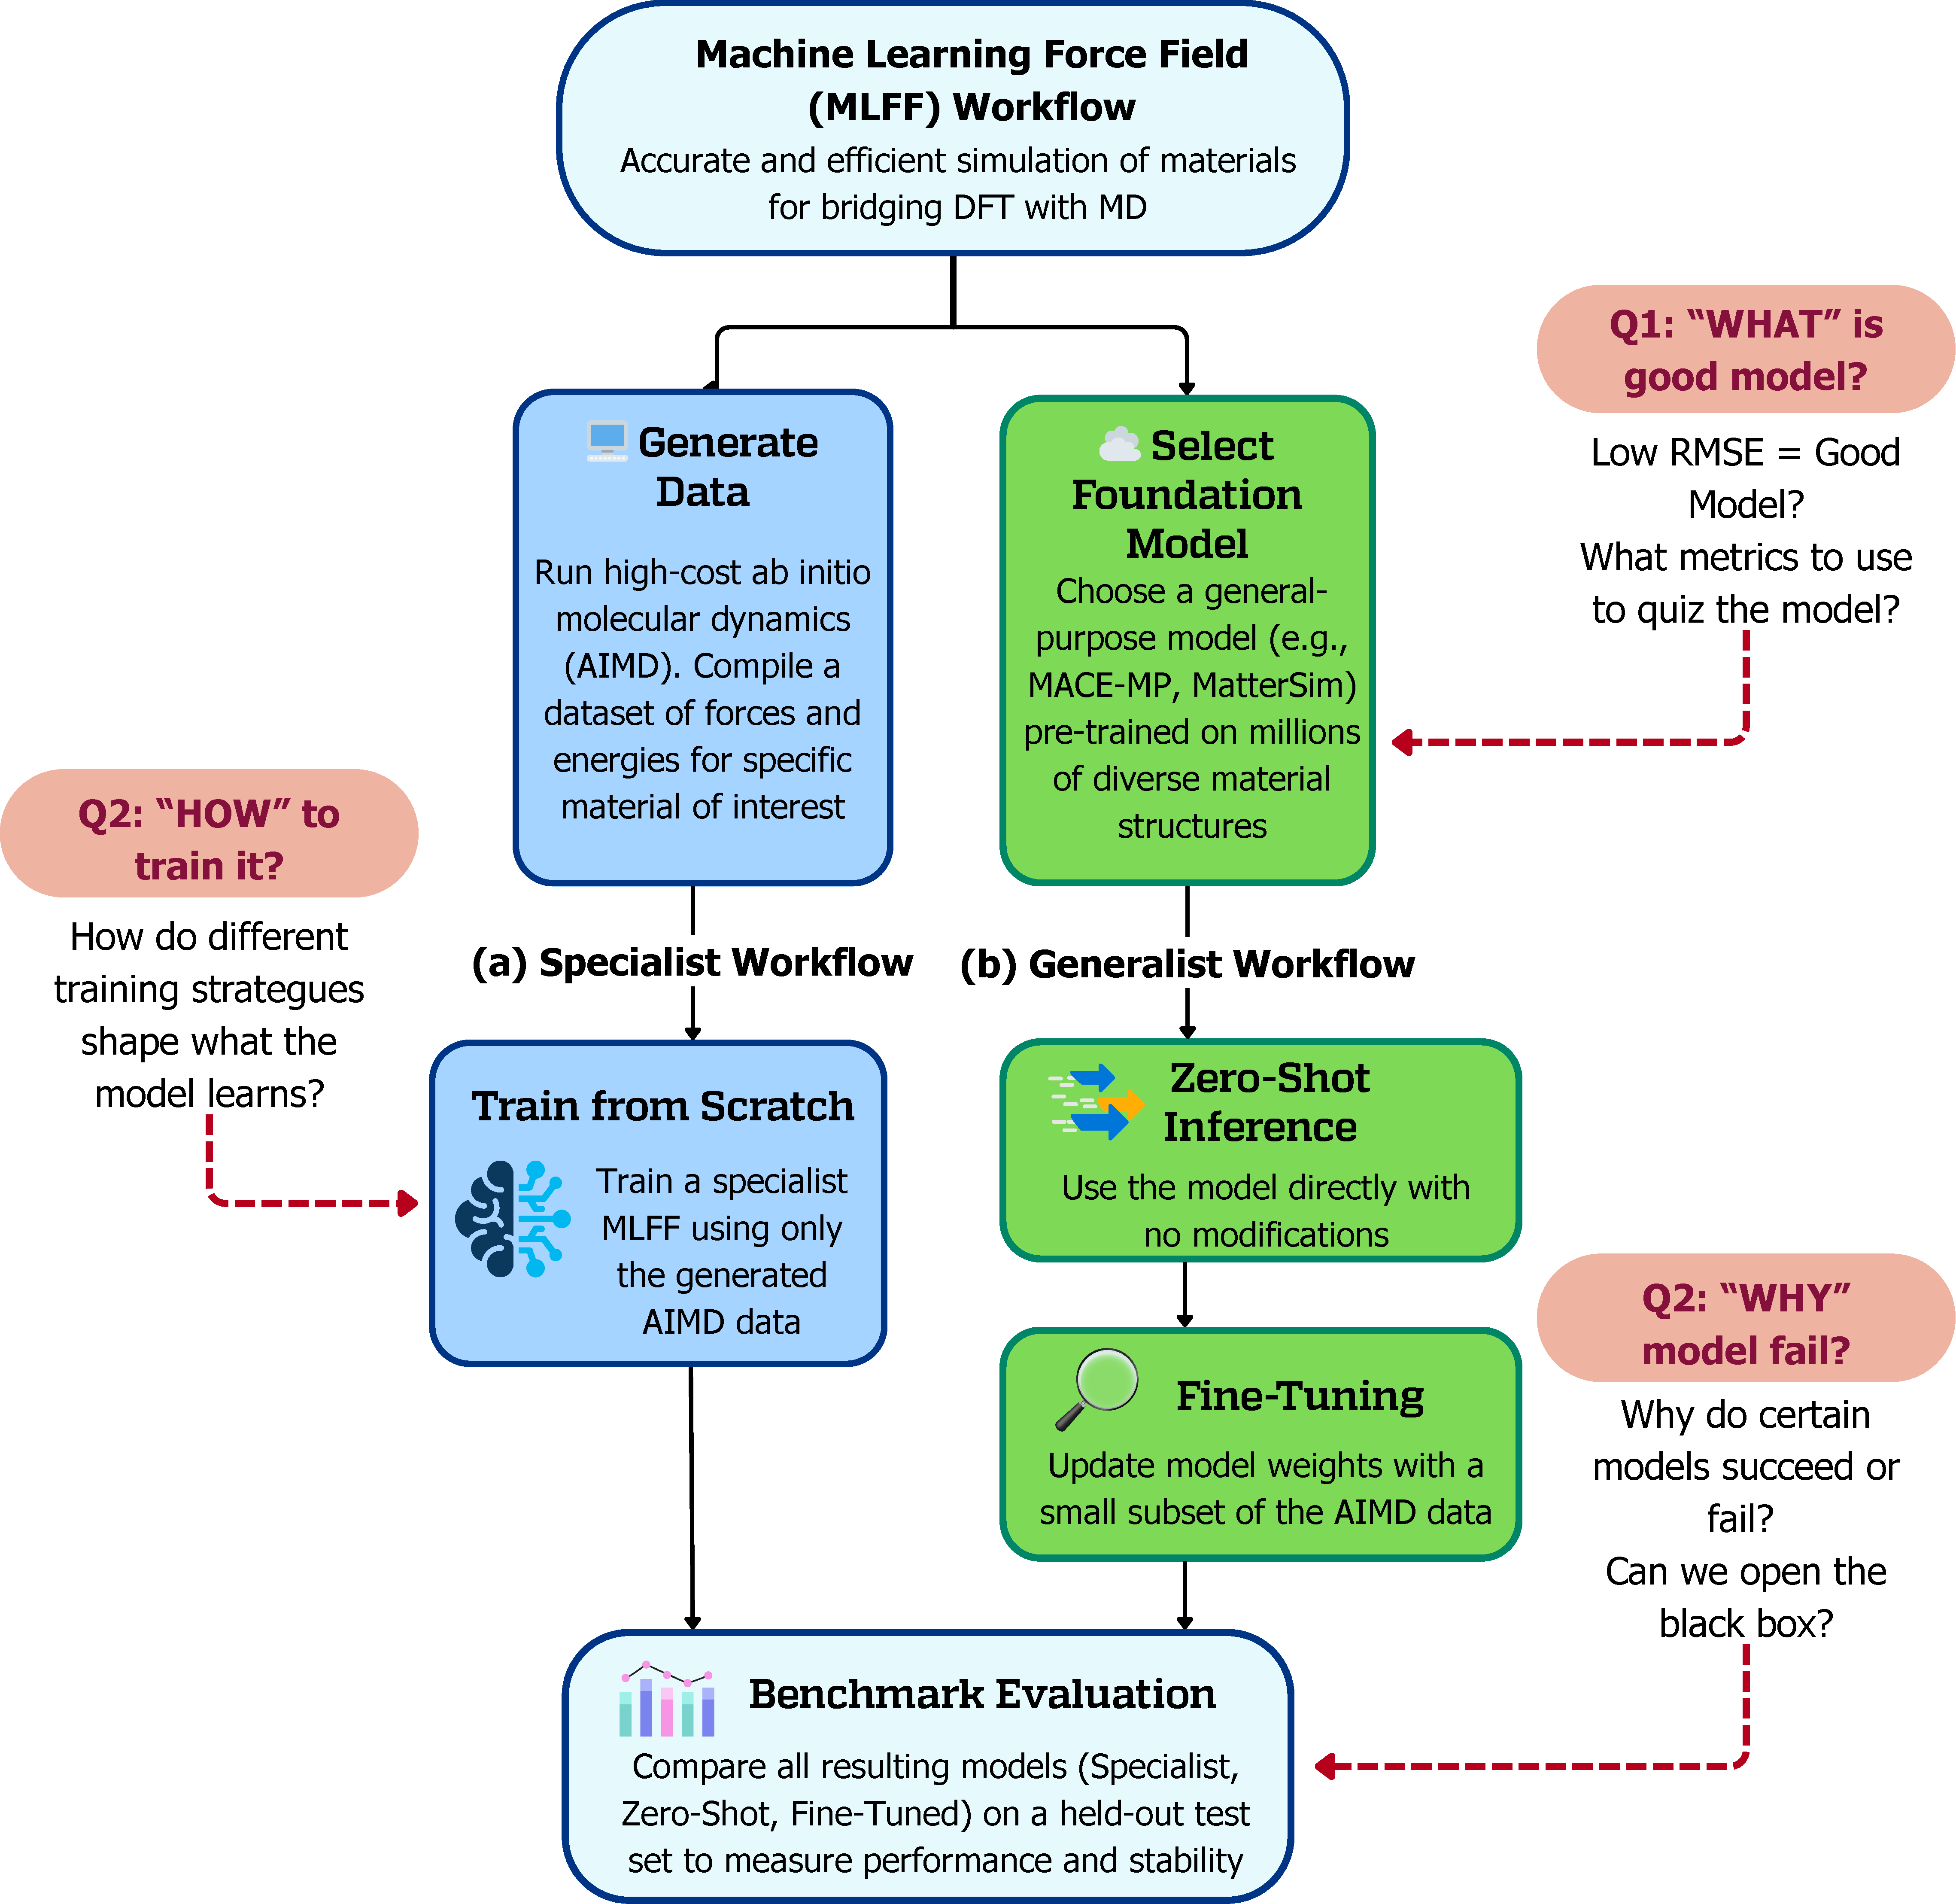
\includegraphics[width=0.7\textwidth]{Fig/NeurIPS2025-AI4MAT-fig1-schematic.pdf}
    \caption{\textbf{Conceptual Workflow Diagram}  illustrating two competing workflows: (a) training a specialist MLFF from scratch, and (b) fine-tuning a generalist foundation model. The diagram highlights the benchmarking questions addressed in this paper.}
    \label{fig:conceptual_diagram}
\end{figure}


\section{Methodology}
We employed a systematic approach to benchmark various Machine-Learned Force Fields (MLFFs) for Cr-doped \ce{Sb2Te3}\footnote{This material system serves as an ideal testbed because its anisotropic van der Waals structure provides distinct migration environments: in-gap diffusion within quintuple layers (representing in-distribution scenarios) and interlayer migration across vdW gaps (probing out-of-distribution regimes). This structural duality enables efficient sampling of diverse configurations—from equilibrium states to high-energy transition states—while addressing technologically relevant processes where both thermodynamic stability and kinetic properties are critical for doping engineering.}, 
comparing specialist models trained from scratch against fine-tuned foundation models. 

\subsection{Data-Generation and Model-Training}
Reference data were generated using density functional theory (DFT) calculations adopting the well-used PBE functional~\citep{perdew_generalized_1996} and comprising roughly 20,000 configurations of a $4\times 2 \times 1$ system of the \ce{Sb2Te3} crystal~\citep{jain2013commentary}. We use a  1~fs timestep  
for a series of \textit{ab initio} molecular dynamics (AIMD) simulations at three temperatures (300~K, 600~K, 1200~K). We employed the MACE architecture for all models, which is a message-passing neural network for the representation of atomic interactions.~\cite{batatia_mace_nodate} 


This paper evaluates four distinct training strategies to benchmark their performance:
\begin{enumerate}
\item \textbf{Scratch}: MACE model trained exclusively on our AIMD dataset
\item \textbf{Foundation}: Pre-trained MACE-MP model used without fine-tuning
\item \textbf{FT-600~K}: Foundation model fine-tuned on 5\% of data from 600~K trajectories
\item \textbf{FT-MultiT}: Foundation model fine-tuned on multi-temperature data from the three temperatures studied
\end{enumerate}

\subsection{Evaluation Framework}
Models were assessed through: (i) Molecular dynamics simulations at 300~K and 600~K to evaluate structural stability and transport properties, (ii) Nudged Elastic Band calculations for migration barriers, and (iii) representation learning analysis using $t$-SNE visualization of physically interpretable descriptors. Performance metrics included force/energy accuracy, dynamic stability, barrier prediction errors, and latent space clustering quality. Detailed computational parameters are provided in the Supplementary Information.

\subsection{SHAP Analysis}
\reviewermap{REV-A6/REV-C13}{done-local}{SHAP methods updated to the audited 150-frame absolute-energy-error surrogate workflow.}
We employed a model-agnostic SHAP workflow to identify SOAP descriptors associated with MACE energy-error behavior. Local atomic environments were encoded using SOAP descriptors (5.0~\AA\ cutoff, $n_{\mathrm{max}}=4$, $l_{\mathrm{max}}=4$), capturing species-resolved radial and angular interactions in Cr-doped \ce{Sb2Te3}. For each MACE variant, gradient-boosted regressors (200 trees, learning rate 0.05, max depth 8) were trained to predict the absolute total-energy error on the audited 150-frame trajectory. TreeSHAP values were then computed for the fitted surrogate models, and surrogate fidelity was assessed with 5-fold cross-validation rather than in-sample $R^2$. We compared the top 50 influential SOAP features across models to identify shared versus model-specific sensitivities in the surrogate error model.


\section{Results and Discussions}

\subsection{Equilibrium Properties: Foundation for Comparison}
We considered four candidate models: a ``zero-shot'' foundation model, a bespoke model trained from scratch, and two fine-tuned variants of the foundation model. As a baseline, we first evaluated their predictive accuracy on static DFT data using standard energy and force RMSE metrics (Table~S1). These metrics already satisfy the typical thresholds for high-quality MLFFs, and the corresponding parity plots show that all models achieve visually indistinguishable agreement with DFT across energies and forces (Fig.~S1). 

Because the RMSE performance converges to similarly strong values, accuracy on equilibrium properties alone cannot reveal the qualitative and quantitative differences between our training strategies. This motivates the need for a more rigorous, physics-based benchmark, namely, assessing the fidelity of each model in molecular dynamics. We, therefore, examined the ability of each model to reproduce thermodynamic, structural, dynamic, and transport properties using MD simulations (Fig.~\ref{fig:ensemble}a). Each model drove a 200~ps trajectory, and all trajectories were subjected to an identical post-processing workflow to quantify their resulting physical properties (Fig.~\ref{fig:ensemble}).

\begin{figure}[ht]
    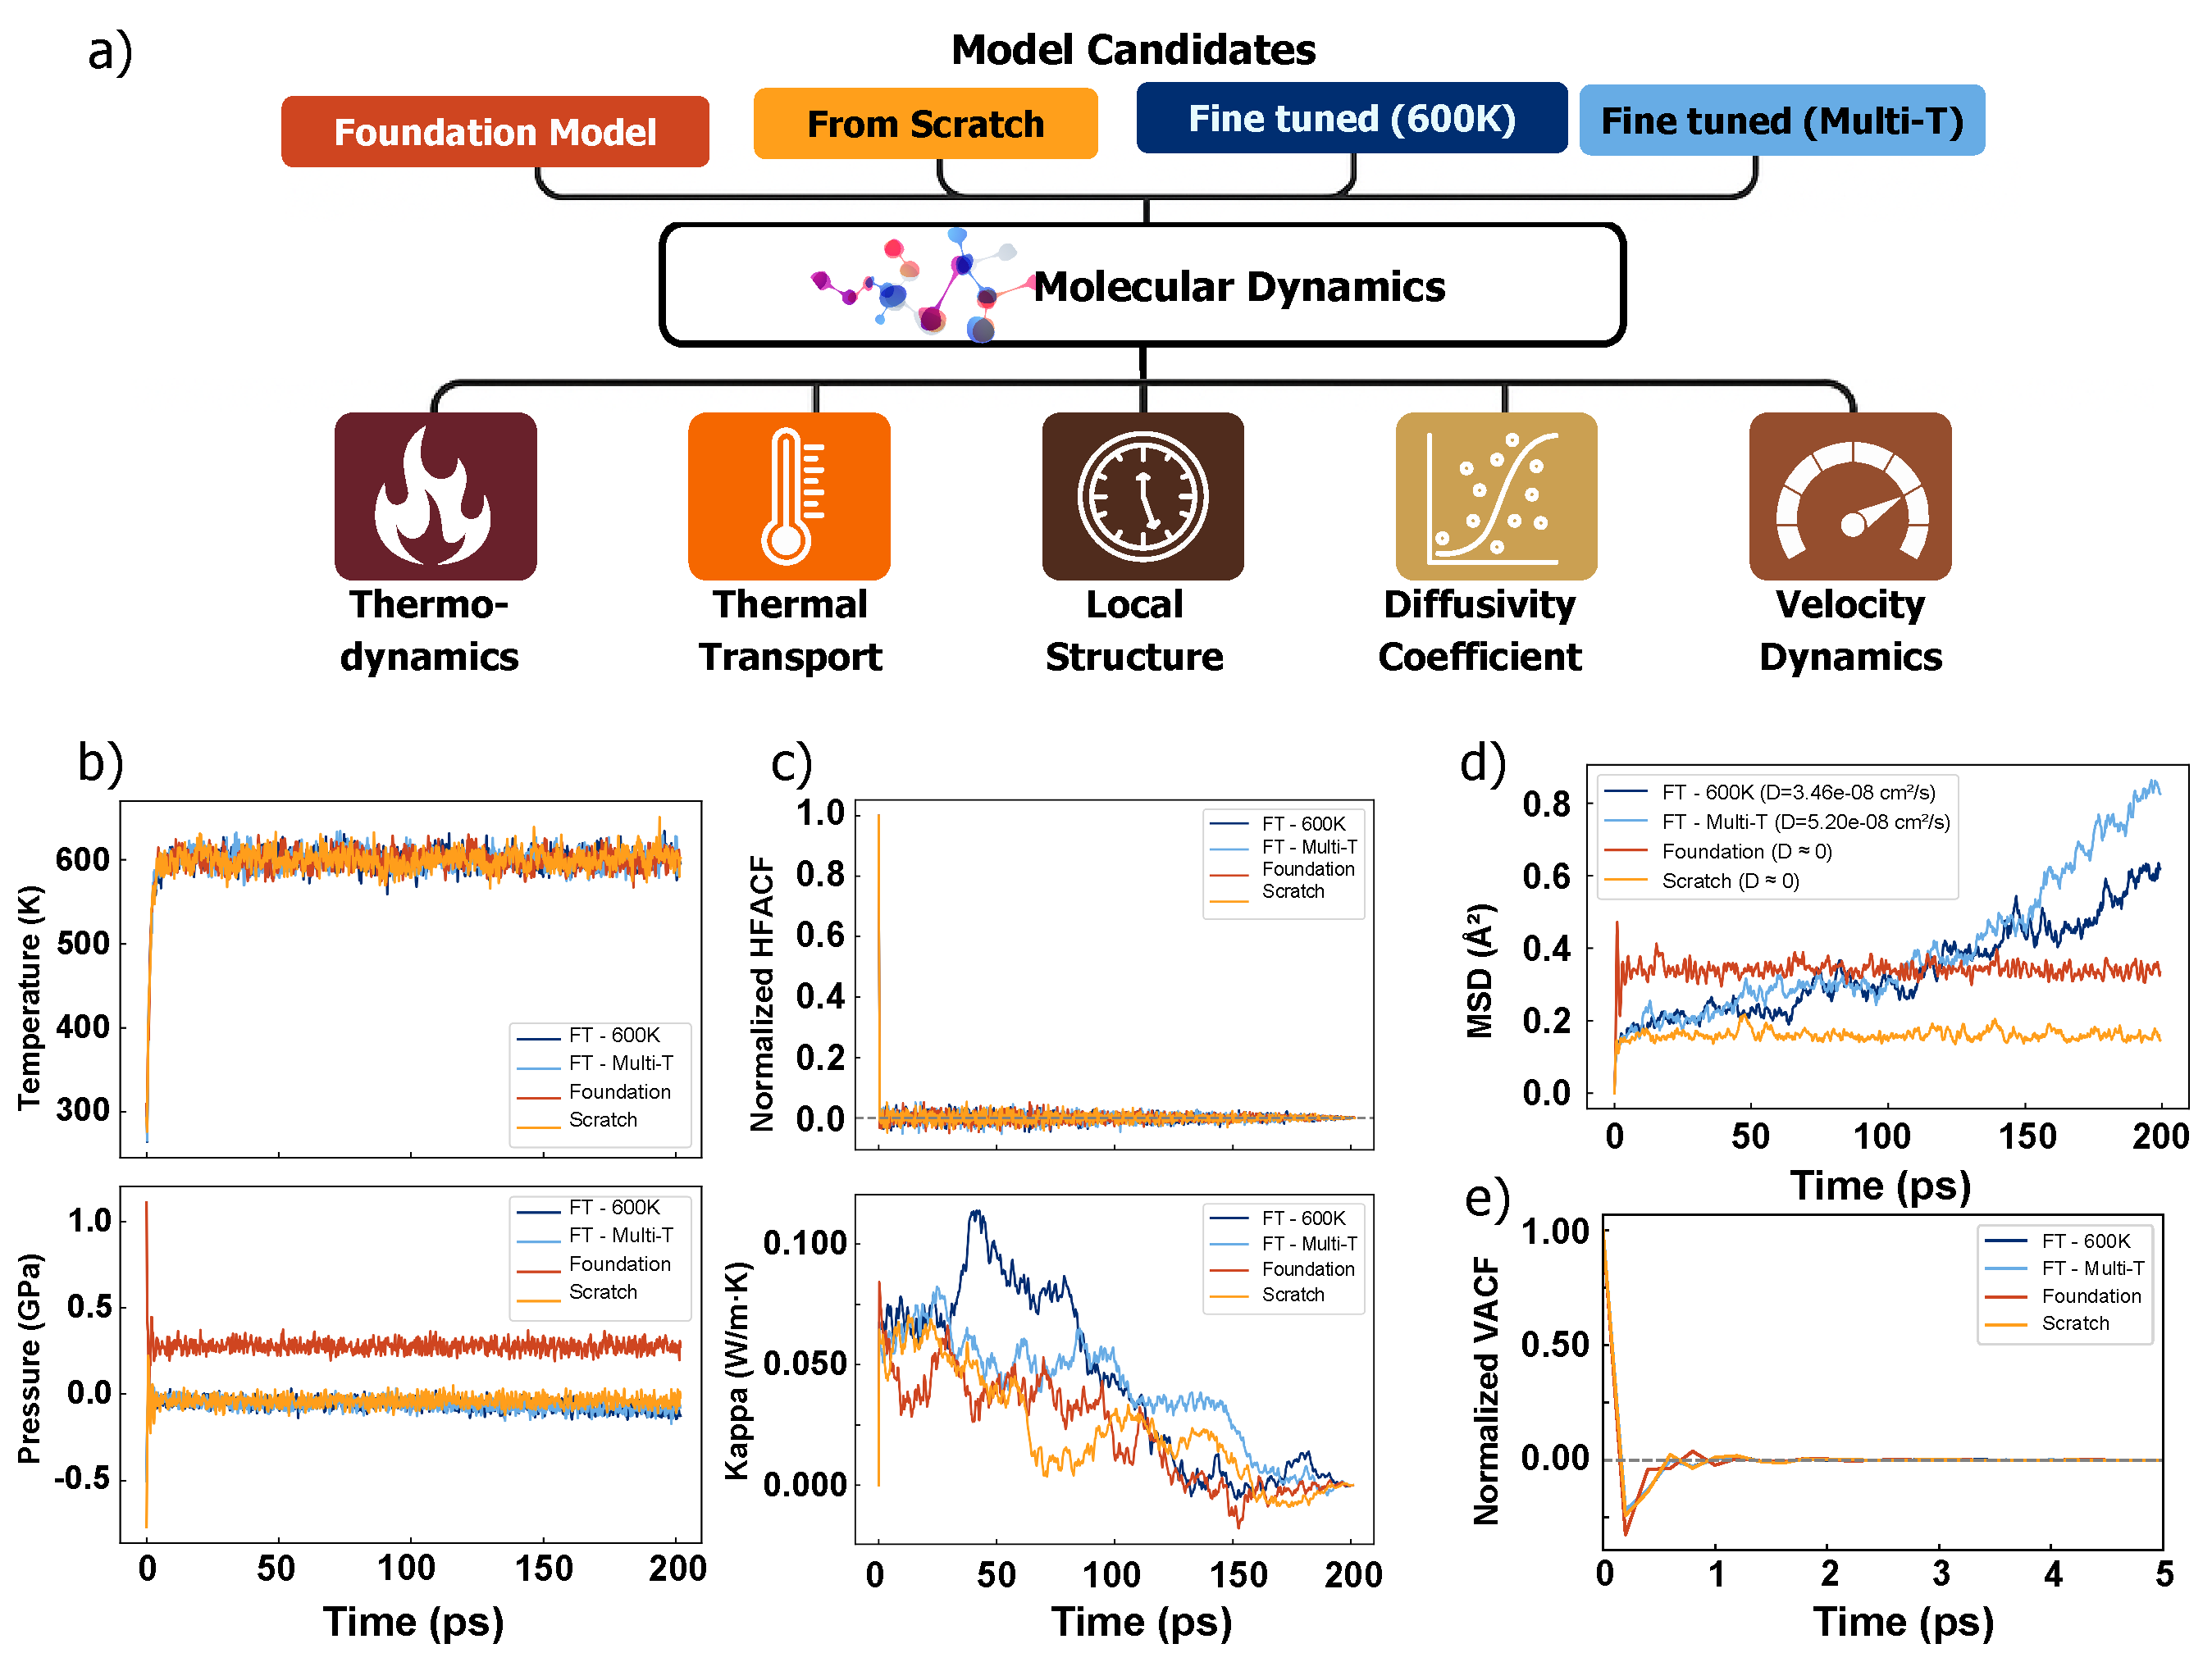
\includegraphics[width=0.8\textwidth]{Fig/NeurIPS2025-AI4MAT-fig2-v2.pdf}
    \centering
    \caption{\textbf{Comprehensive Benchmarking of MLFF Performance in Molecular Dynamics Simulations.} (a) A schematic of the unified evaluation protocol. Four candidate models (a zero-shot foundation model, a bespoke model trained from scratch, and two fine-tuned variants) were used to drive a 200~ps MD simulation. The resulting trajectories are then subjected to a uniform set of post-processing analyses to evaluate key physical properties. (b) Thermodynamic stability, demonstrated by the evolution of temperature and pressure over the simulation, remain acceptably stable around their target values for all models. (c) Thermal transport properties, showing the Heat Flux Autocorrelation Function (HFACF) and its running integral to compute thermal conductivity ($\kappa$).  (d) The Mean Squared Displacement (MSD), used to assess atomic mobility and calculate the diffusion coefficient. (e) The Velocity Autocorrelation Function (VACF), which describes the system's underlying dynamics.}
    \label{fig:ensemble}
\end{figure}

All MACE models (Foundation, Scratch, FT-600K, FT-Multi\_T) successfully reproduce the equilibrium structure of Cr-doped Sb$_2$Te$_3$, with RDF analysis showing excellent agreement with the AIMD reference (``ground truth'') across all atomic pair correlations (Fig.~S2). Fig.~S2 includes a structural schematic of the local environment around Cr and full radial distribution functions (RDFs) for all models, confirming that each training strategy preserves the characteristic nearest-neighbor and second-shell coordination features at 600~K. While all models maintain stable thermodynamic ensembles at 600~K (Fig.~\ref{fig:ensemble}c), the zero-shot foundation model shows a persistent pressure offset, likely originating from its exposure to predominantly 0~K equilibrium structures rather than configurations extant at finite-temperatures.

\reviewermap{REV-C9}{pending-cluster}{Long-run MD transport values must be replaced by the corrected 100000-step workflow before final submission.}
Despite similar performance on local structural (RDF) and short-time dynamic (VACF) properties (Fig.~\ref{fig:ensemble}e), the models diverge in their preliminary predictions of long-timescale transport phenomena. In the current short-run analysis, fine-tuned models predict higher diffusion coefficients than both foundation and scratch models (Fig.~\ref{fig:ensemble}d), with the multi-temperature fine-tuned variant showing the largest enhancement. Because diffusion and thermal-transport coefficients are sensitive to sampling length and trajectory health, the final analysis will replace these values with the corrected long-run MD workflow [PLACEHOLDER: corrected 100000-step MD diffusion and thermal-conductivity values]. If the ranking is unchanged, we will retain the interpretation that high-temperature training exposure can flatten the effective PES; if the ranking changes, the text and figure will be regenerated from the audited workflow.

Notably, thermal conductivity calculations reveal differences in the way that the  models capture collective vibrational modes. The foundation model's thermal conductivity decays rapidly toward zero, failing to sustain the long-range phonon correlations characteristic of the crystalline structure. In contrast, models trained (or fine-tuned) on system-specific data maintain these correlations, although the 600K-only model exhibits an anomalous peak suggesting structural instability in the potential. These results demonstrate that validating MLFFs solely on static structures and short-time dynamics is insufficient; a comprehensive assessment must include transport properties that probe long-range, collective phenomena.




\subsection{Non-Equilibrium Diffusion Pathways: The Critical Test of Generalization}

A rigorous test of the generalizability of a machine learning force field extends beyond its ability to reproduce thermodynamic properties. It must also accurately describe the potential energy surface (PES) in regions far from the training data's energetic minima, such as the high-energy transition states that govern kinetic processes. To this end, we evaluated the performance of our MACE model on the challenging task of predicting the diffusion barrier for a fundamental migration event in the Cr-doped Sb$_2$Te$_3$ system. This task is substantially more demanding than constant-temperature MD simulations (\textit{e.g.,} at 600~K), as it requires the model to capture not only accurate energies but also the subtle curvature of the PES at a first-order saddle point, which represents a particularly stringent test of the model's learned representation of interatomic interactions.

\begin{figure}[ht]
    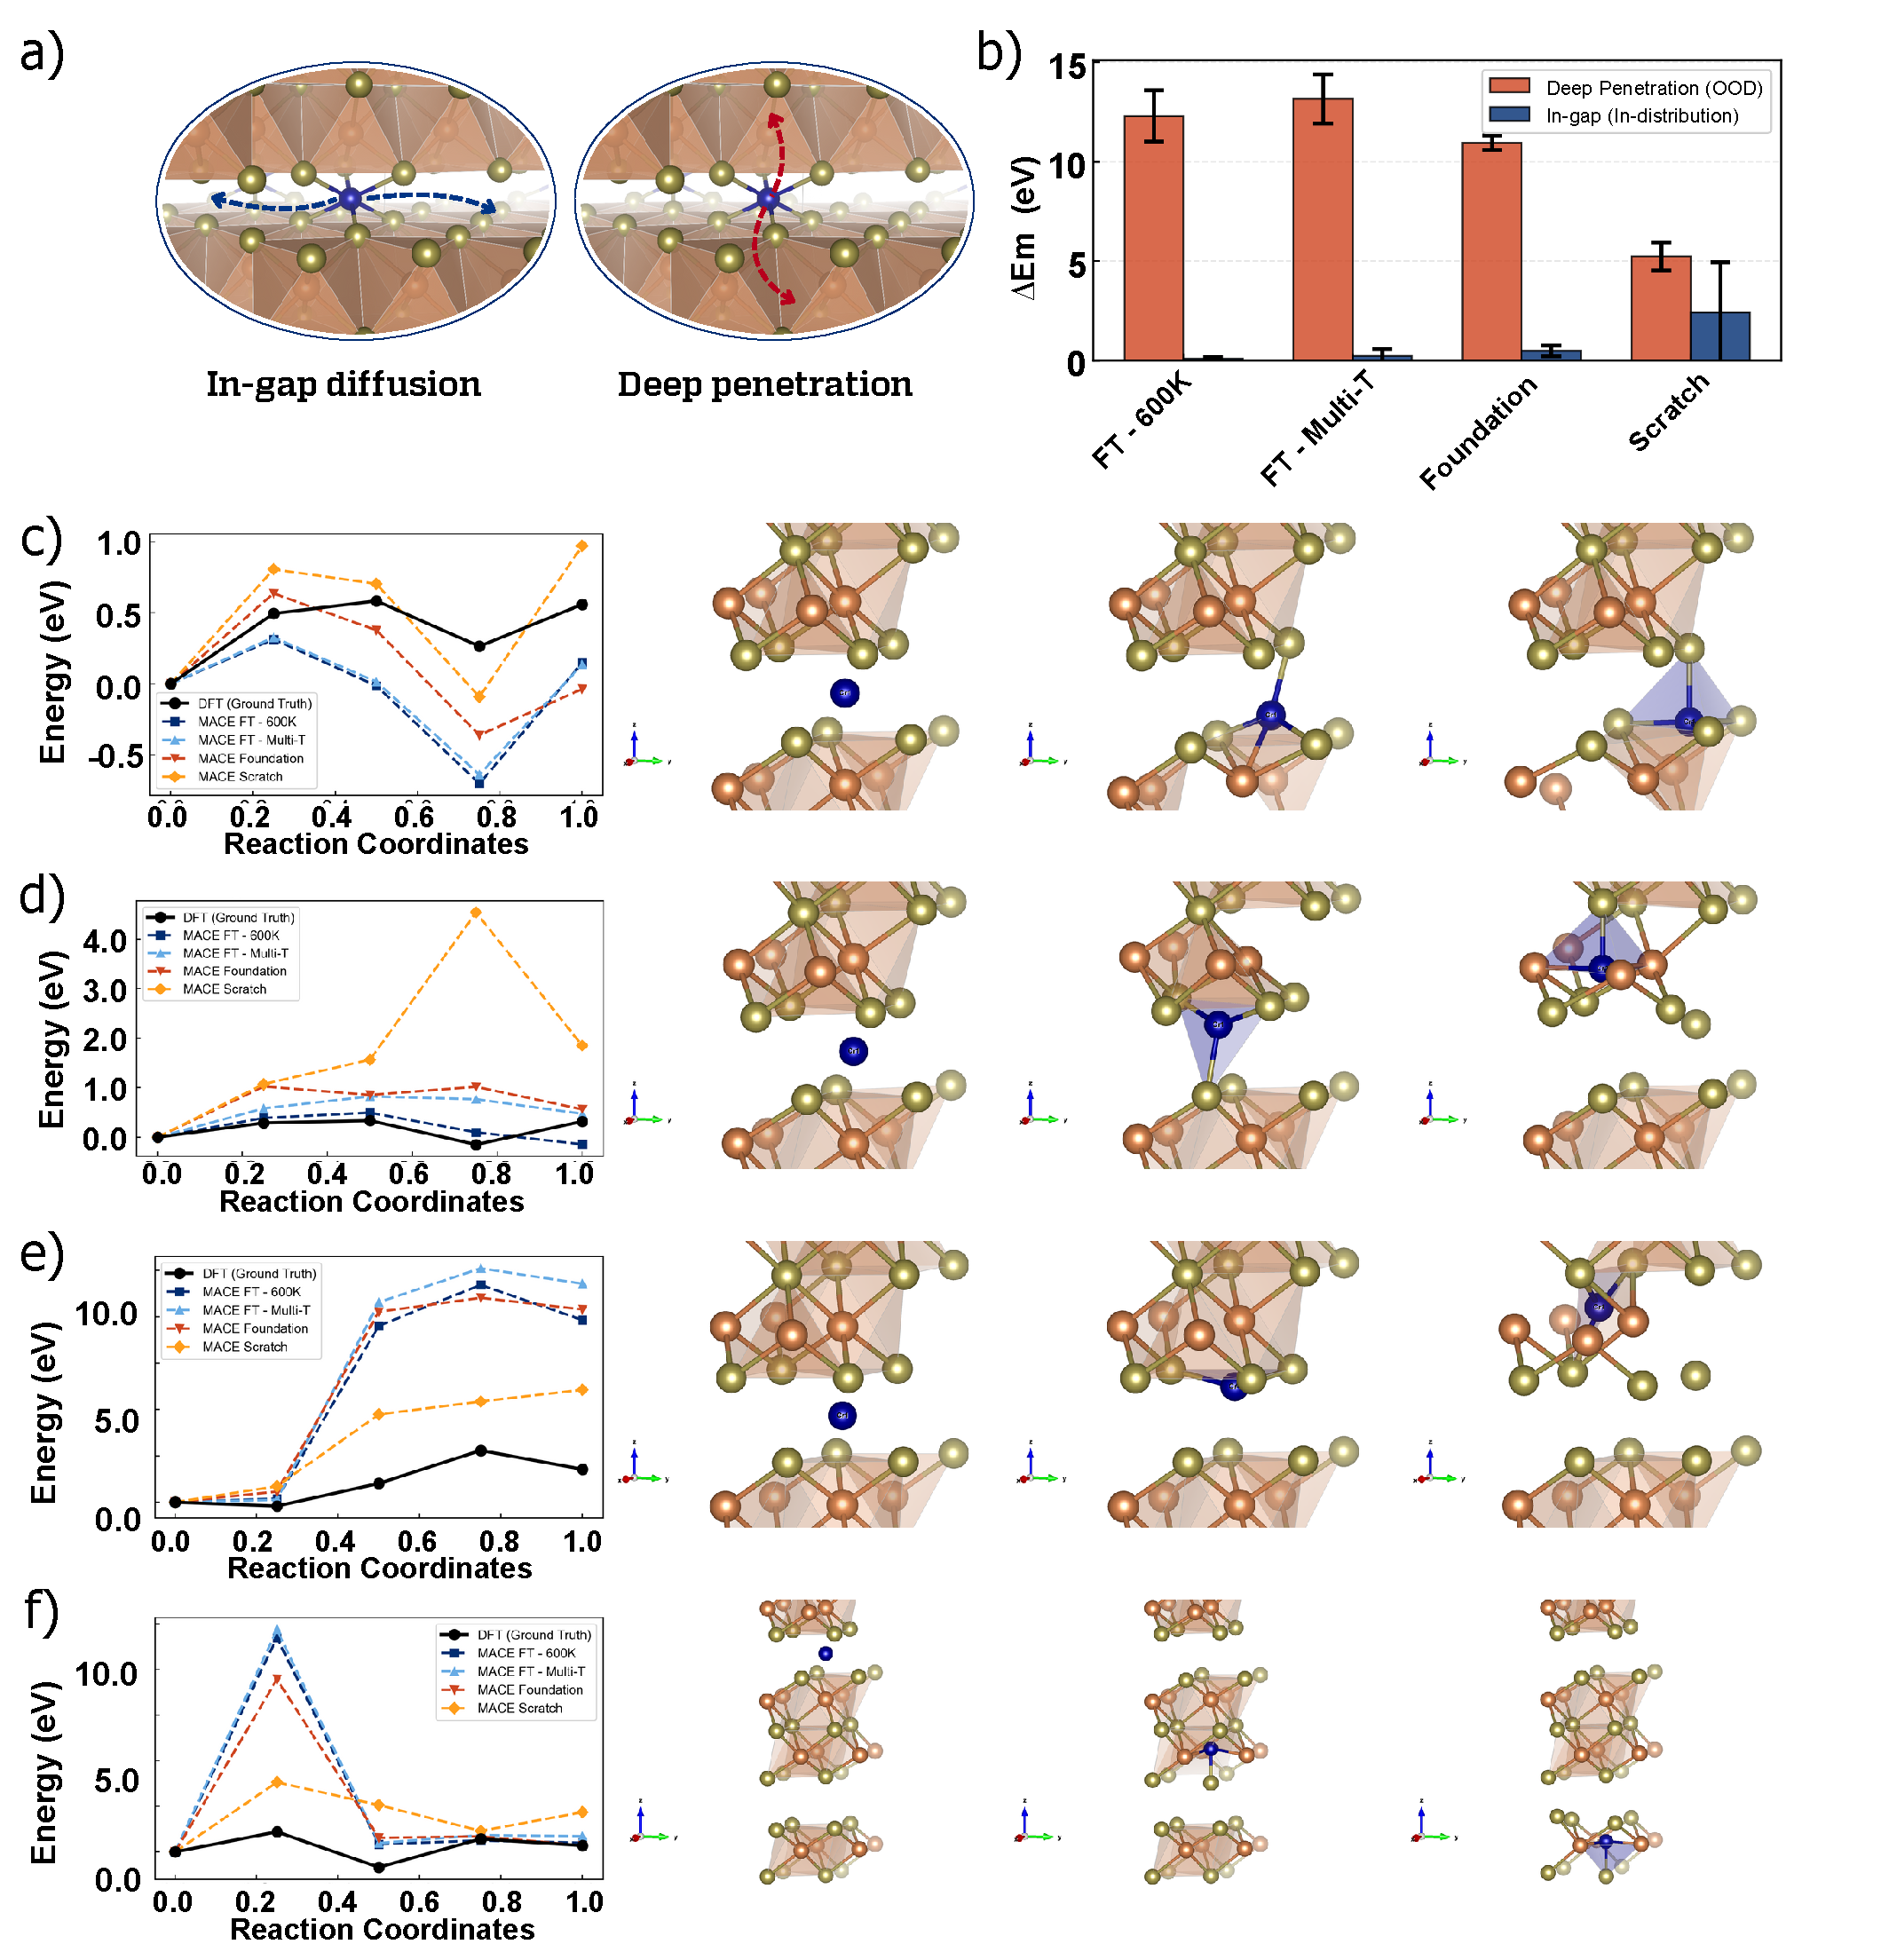
\includegraphics[width=0.8\textwidth]{Fig/NeurIPS2025-AI4MAT-figure4-v2.pdf}
    \centering
    \caption{\textbf{Comparative analysis of MLFF training strategies for predicting atomic migration barriers.} (a) Schematic illustration of the simulated Cr atom migration pathway between two stable sites within the Sb$_2$Te$_3$ bilayer. (b) Bar plot showing the migration energy prediction errors for various models, spanning bespoke training to advanced active- learning approaches. (c--f) Comparison of the minimum energy pathway (MEP) profiles for the Cr migration process. The solid black line denotes the ground-truth DFT reference data, while dashed lines represent predictions from MACE models trained with different strategies. 
    % The from-scratch model (orange) significantly underestimates the energy scale, whereas the zero-shot foundation model (red) captures the qualitative shape but yields a quantitatively ``softened'' profile. Targeted fine-tuning with 600 K data (dark blue) substantially reduces the error and closely reproduces the DFT barrier, highlighting the importance of task-specific data in refining the potential energy surface and achieving high-fidelity kinetic predictions.
    }
    \label{fig:barrier}
\end{figure}


\subsubsection{Local Migration Events}

To perform a direct and controlled evaluation of the learned Potential Energy Surface (PES) for each model, we used the minimum energy pathway (MEP) obtained from our reference DFT Nudged Elastic Band (NEB) calculations as a fixed geometric trajectory. By calculating the single-point energy for each of these pre-defined images, we can decouple the model's energetic accuracy from its structural relaxation behavior, providing a direct probe of its ability to describe the reaction pathway.

\reviewermap{REV-A1}{partial}{Fig. 3d is fixed-geometry DFT-path scoring; current 1-4 DFT reference candidate is 0.336050 eV; Foundation fixed-path error is +0.688246 eV.}
Here the DFT NEB path is used as a fixed geometric reference. For the in-gap pathway labeled 1--4 in the audited workflow, the current DFT candidate barrier is 0.336~eV; this value will be retained only after the restarted QE NEB run satisfies the stated convergence criterion, otherwise the table and plot will be regenerated from the converged restart. The results in Fig.~\ref{fig:barrier}d therefore measure a fixed-path scoring task: each MLFF is asked to assign energies to the same DFT-relaxed images, so the comparison probes energetic fidelity along an externally supplied trajectory rather than the model's ability to discover the path.
The two baseline strategies, training from scratch and using the zero-shot foundation model, demonstrate the fundamental challenges of specialization and generalization. The MACE Scratch model, despite being trained on a comprehensive in-house dataset, exhibits a catastrophic failure in predicting the energy barrier, overestimating the activation energy by over 4~eV, an unacceptably high amount. This is a classic signature of poor extrapolation. Even with tens of thousands of AIMD frames, the high-energy, low-probability configurations corresponding to the transition state are insufficiently sampled. Consequently, the model overfits to the more prevalent, near-equilibrium states and fails dramatically when asked to evaluate this critical, out-of-distribution, rare event.

Conversely, the MACE Foundation model provides a qualitatively plausible fixed-path profile, capturing the smooth, convex shape of the energy barrier. However, it is quantitatively inaccurate on this fixed DFT trajectory: the audited value is 1.024~eV, corresponding to an error of +0.688~eV relative to the current DFT candidate barrier. We therefore describe the zero-shot model as insufficient for quantitative fixed-path barrier prediction in this system, not as unstable in all NEB settings. The overestimated barrier is consistent with a broader concern for universal MLIPs: pretraining can provide robust qualitative physics while still missing system-specific curvature along a rare-event pathway~\citep{deng2025softening}. The pronounced failures of the baseline strategies motivate fine-tuning, but the distinction between fixed-path scoring and self-consistent NEB optimization is essential for interpreting the comparison.


% \paragraph{Further Testing Different Trajectories}

To probe the generalization capabilities of the different MLFF training strategies, we evaluated their performance on two distinct Cr migration pathways (Fig.~\ref{fig:barrier}a) with fundamentally different characteristics. The first pathway, \emph{in-gap diffusion}, involves Cr migration within the vdW gap between Sb$_2$Te$_3$ quintuple layers, with low energy barriers and configurations similar to the training data, thereby testing interpolative accuracy.

In contrast, the second pathway, \emph{deep penetration}, requires the Cr atom to move vertically from the vdW gap and penetrate directly into the interior of a QL, ultimately reaching a deeply buried site within the layer. This migration path is associated with significantly higher energy barriers and accesses high-distortion configurations that are not well-represented in the training data, making it an out-of-distribution (OOD) scenario with potentially more metastable configurations along the pathway. Testing both pathways allows us to evaluate model accuracy on familiar configurations and extrapolative power in challenging regions of the configuration space.


\subparagraph{In-Gap Diffusion: A Test of Interpolative Accuracy}

For the in-gap diffusion pathway (Fig.~\ref{fig:barrier}c--d), where the Cr atom moves within the vdW gap or just shallowly penetrates the interface, the atomic environments along the minimum energy path (MEP) are reasonably similar to the near-equilibrium states sampled during the AIMD simulations. In this regime, the performance hierarchy is clear. The fine-tuned models, particularly MACE FT--600K, demonstrate excellent agreement with the DFT reference, accurately predicting both the thermodynamic endpoints and the kinetic barrier (Fig.~\ref{fig:barrier}d). This success highlights that, when the task lies within the domain of the training data, fine-tuning effectively ``sharpens'' the generalist foundation model's potential energy surface (PES) to capture system-specific details. In contrast, the MACE Scratch model, despite being trained on the same data, fails significantly, underscoring its inability to learn the subtle energy differences required to resolve the transition state from a limited dataset.

\subparagraph{Deep Penetration: A Test of Extrapolative Robustness}

The ``deep penetration'' pathway provides a much more stringent test of model robustness. This path involves significant lattice distortion as the Cr atom pushes its way through the covalently bonded quintuple layer (QL), creating atomic environments that are far from those seen in the training data (Fig.~\ref{fig:barrier}a).

While the fine-tuned and foundation models remain accurate for the stable initial and final states (an interpolative task), they fail catastrophically in predicting the energy of the transition state, overestimating the barrier by a large margin. This is a classic example of out-of-distribution failure, where the inductive biases learned from near-equilibrium data do not generalize to highly distorted, high-energy configurations. The models have learned to be a ``materials expert'' for stable structures but remain a ``naïve physicist'' for unseen, strained states.

\reviewermap{REV-A3}{pending-cluster}{Deep-penetration interpretation requires multi-seed and restarted QE NEB confirmation before ranking models.}
The MACE Scratch model, which performed least well of the four models on the in-gap pathway, yields the lowest barrier error for this out-of-distribution task (Fig.~\ref{fig:barrier}e, f). We do not interpret this isolated result as evidence that the scratch model is physically superior. Rather, because the deep-penetration path samples highly strained configurations and the current DFT NEB trajectories are still being consolidated, this comparison is treated as a seed- and path-stability question. The completed analysis will report the multi-seed barrier distribution and the converged QE reference values for these paths [PLACEHOLDER: multiseed deep-penetration barrier errors and convergence status]. Until those checks are complete, the result supports the narrower conclusion that equilibrium accuracy does not reliably predict rare-event barrier accuracy.

\paragraph{The Critical Role of Task-Specific Fine-Tuning}
\reviewermap{REV-A5}{pending-cluster}{Add Scratch-5\% random-initialization control trained on the same approximately 1000 configurations as FT-600K.}

The dramatic improvement seen in the fine-tuned models especially for the in-gap diffusion task (Fig.~\ref{fig:barrier}b) underscores the necessity of specializing the foundation model's knowledge. The MACE FT--600K model, fine-tuned specifically on data generated at the target temperature of the migration event, achieves remarkable accuracy, with a barrier error of only 0.16~eV. This demonstrates that targeted fine-tuning effectively ``sharpens'' the softened PES of the foundation model. By providing a small but highly relevant set of in-domain data, we enable the model to learn the specific local atomic interactions required to accurately resolve the transition state structure and energy.

Intriguingly, the MACE FT--Multi-T model, which was fine-tuned on a larger and more diverse dataset spanning multiple temperatures, yields a less accurate barrier than the model trained at a specific temperature, here 600~K. While its predictions for the initial and final states (the thermodynamic endpoints) are accurate, its description of the kinetic barrier is a compromise, retaining some of the ``softened'' character of the original foundation model. This leads to an important insight: for MLFFs, more data is not axiomatically better. The relevance of the fine-tuning data to the specific task is paramount. Because this claim depends on whether training configurations overlap with the benchmark path, we now pair the comparison with a grouped-split protocol and nearest-neighbor SOAP/RMSD audit [PLACEHOLDER: train--test proximity values for FT--600K and FT--Multi-T]. We are also adding a randomly initialized Scratch-5\% control trained on the same approximately 1000 configurations as FT--600K to separate the effect of data volume from the effect of the foundation prior [PLACEHOLDER: Scratch-5\% control errors]. These findings collectively highlight a critical challenge in the practical application of MLFFs. The failure of the from-scratch model illustrates the difficulty of adequately sampling rare events, while the inaccuracies of the foundation model reveal the limitations of a purely generalist approach.

The success of targeted fine-tuning points the way forward, but the divergent results of the 600~K and Multi-T models prove that the data selection process is non-trivial. This motivates the need for more advanced methods, such as the uncertainty-guided active learning explored in our work, which can intelligently identify and acquire the most informative data to improve model robustness and accuracy in a data-efficient manner.


\subsubsection{NEB Stability as an Additional Robustness Criterion}
\reviewermap{REV-A1}{partial}{Define Fig. 3d and SI Fig. S3 as different NEB operators and report them side-by-side.}
Beyond evaluating the models on pre-computed DFT NEB geometries, we also assessed a distinct task: whether each MLFF can independently optimize an NEB band without being given the DFT-relaxed path. Formally, Fig.~\ref{fig:barrier}d evaluates a fixed-path operator, $E_M(x_i^{\mathrm{DFT}})$, whereas Fig.~S3 evaluates a self-consistent MLFF-NEB operator, $x_i^{M,*}=\mathrm{NEB}(M;x_0,x_N)$ followed by $E_M(x_i^{M,*})$. The 0.41~eV value in Fig.~S3 is therefore the MACE Foundation model's self-consistent MLFF barrier on its own optimized path, not a second DFT reference and not a contradiction of the +0.688~eV fixed-path error in Fig.~\ref{fig:barrier}d. In sharp contrast, the scratch, FT-600K, and FT-MultiT models all exhibit explosive behavior in this self-consistent optimization, where a rapid increase in the maximum force triggers early termination. Thus, fixed-path scoring measures energetic accuracy on a common DFT geometry, while self-consistent MLFF NEB measures optimization stability and qualitative path robustness.

\begin{figure}[ht]
    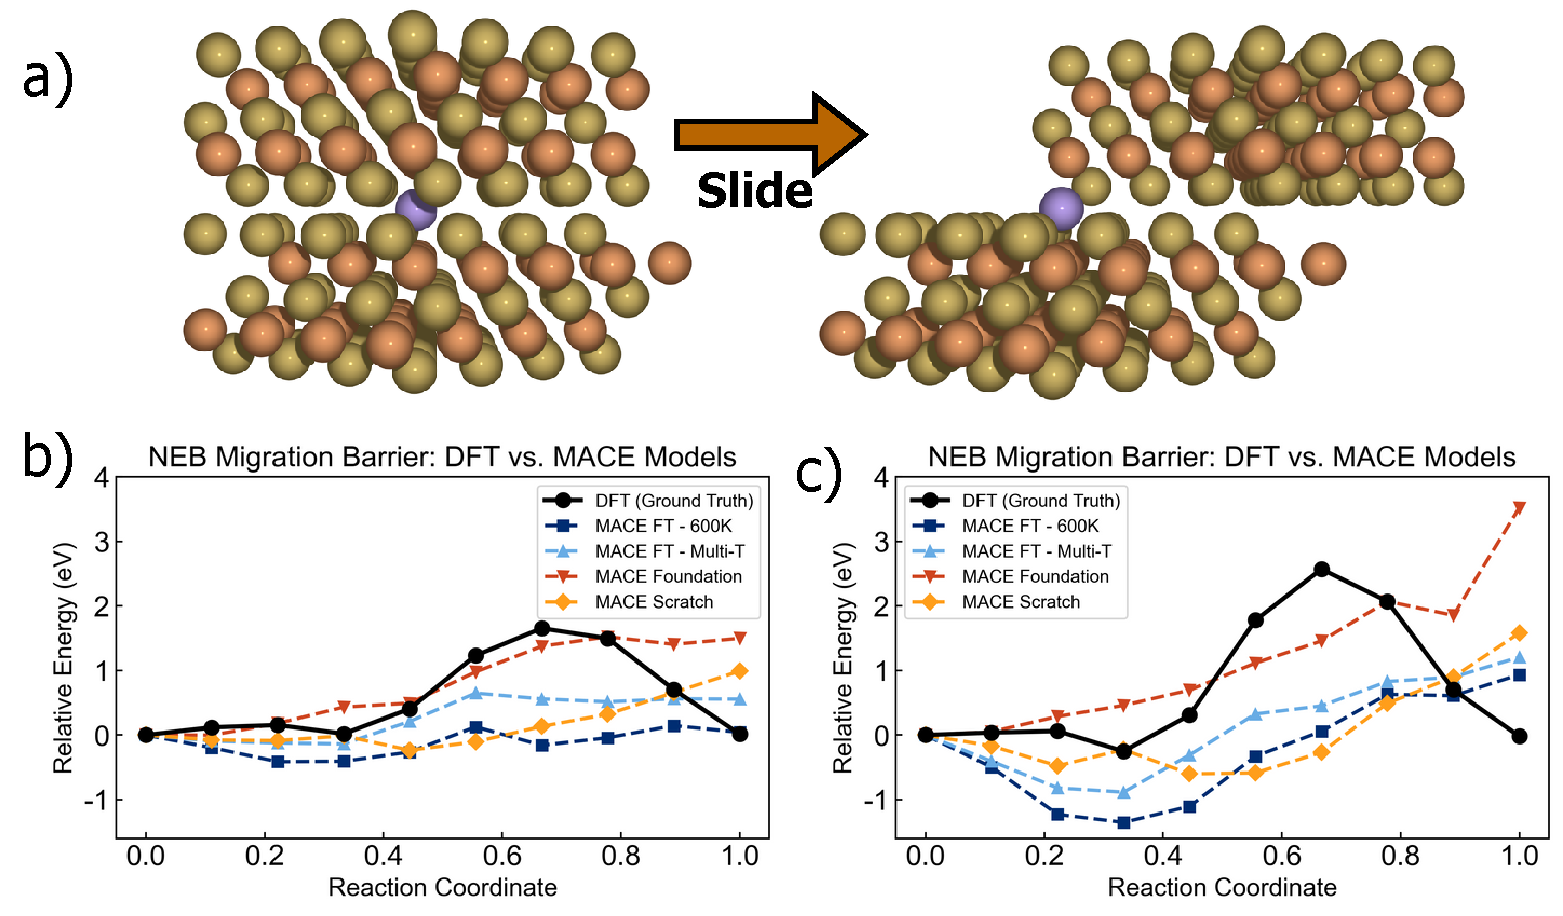
\includegraphics[width=0.6\textwidth]{Fig/NeurIPS2025-AI4MAT-figure5.pdf}
    \centering
    \caption{\textbf{Evaluation of MACE models on collective lattice displacement: interlayer sliding in Sb$_2$Te$_3$.} (a) Schematic illustration of the bilayer sliding process in Sb$_2$Te$_3$, where the top layer (yellow/orange atoms) slides relative to the bottom layer along the crystallographic direction. The purple sphere indicates the position of a Cr dopant when present. (b) Energy barriers for interlayer sliding in pristine Sb$_2$Te$_3$ as calculated by DFT (black, ground truth) and various MACE models. The reaction coordinate represents the normalized sliding distance from the initial to final configuration. (c) Energy barriers for the same sliding process in Cr-doped Sb$_2$Te$_3$.}
    \label{fig:sliding_results}
\end{figure}



\subsection{Interlayer Sliding: Probing Robustness to Non-Local, Collective Displacements}

Having tested the models' response to local, high-distortion events, we evaluated their robustness to a different class of out-of-distribution challenge: large-scale, collective lattice displacements. To this end, we simulated the shearing of one Sb$_2$Te$_3$ layer relative to another, a process governed by the subtle corrugations of the interlayer vdW potential energy surface (Fig.~\ref{fig:sliding_results}a). This task is particularly challenging for MLFFs as the local atomic environment of any given atom changes only minimally, while the global configuration undergoes a significant transformation that crosses periodic boundaries. The configurations along this sliding path were not present in the training data.

We first examined the case of pure, undoped Sb$_2$Te$_3$ (Fig.~\ref{fig:sliding_results}b). The results reveal a clear trade-off between the models. The MACE Foundation model provides the most reasonable estimate of the energy barrier's shape and magnitude, suggesting its vast pre-training on bulk crystals has endowed it with a better implicit understanding of such periodic, mechanical deformations. However, it fails to maintain translational symmetry, incorrectly predicting the final state to be higher in energy than the identical initial state. This energy drift is a clear artifact, indicating a failure to perfectly respect the periodic nature of the simulation cell under large displacements. The MACE Scratch model exhibits a similar version of this artifact.

In contrast, the fine-tuned models (MACE FT--600K and Multi-T) significantly underestimate the energy barrier. This suggests a compelling hypothesis: the process of fine-tuning, while ``sharpening'' the PES for local chemistry around the Cr dopant, has degraded the model's learned representation of the weaker, long-range interlayer physics inherited from the foundation model. The optimization has prioritized local accuracy at the expense of non-local, collective interactions.

This trend is largely mirrored in the Cr-doped system (Fig.~\ref{fig:sliding_results}c), confirming that this is a fundamental behavior of the models rather than an effect specific to the dopant. The failure of all models to perfectly capture both the barrier height and the endpoint periodicity highlights a key limitation of local-descriptor-based MLFFs. Phenomena like shearing, stacking faults, and dislocation glide are inherently non-local. While the models excel at describing local bonding and coordination, they can struggle to enforce long-range physical constraints that extend beyond their cutoff radius. This further underscores the need for careful validation when using standard MLFFs to study mechanical properties and points towards future work in developing training sets that explicitly include these collective deformation modes or exploring architectures designed to capture long-range physics more effectively.

\subsection{Representation Learning Analysis}

To elucidate the origins of the observed performance differences, we conducted a multi-faceted analysis of the learned representations. We projected high-dimensional atomic environment descriptors from each model's 600~K MD trajectory onto a two-dimensional space using two complementary techniques: $t$-distributed stochastic neighbor-embedding ($t$-SNE)~\citep{maaten2008visualizing} to assess representational dissimilarity, and Potential of Heat-diffusion for Affinity-based Trajectory Embedding (PHATE)~\citep{moon2019visualizing} to reveal the underlying geometric structure of the system's dynamics (Fig.~\ref{fig:tsne-phate}).

The $t$-SNE projection (Fig.~\ref{fig:tsne-phate}a) suggests that models trained with different strategies produce qualitatively distinct encodings. The MACE Foundation and MACE Scratch models occupy separated regions in the projection, while the two fine-tuned models occupy an intermediate region. Because low-dimensional embeddings can amplify or suppress apparent separation, we use these plots as qualitative diagnostics and report quantitative checks in the original descriptor space. In the audited analysis, the original 6191-dimensional Euclidean silhouette score is 0.333, while z-scoring the original features gives a silhouette score of -0.019; the projected baselines are $0.397\pm0.027$ for $t$-SNE and 0.473 for PHATE. These values support representational differences, but they do not by themselves prove a unique mechanistic cause.

While $t$-SNE shows \textit{that} the representations are different, PHATE reveals \textit{why} it matters for physical prediction. The PHATE projection (Fig.~\ref{fig:tsne-phate}b) maps the continuous time-evolution of the system to a low-dimensional ``dynamical manifold,'' an arc-like structure whose geometry is intrinsically linked to the potential energy surface (Fig.~\ref{fig:tsne-phate}c). Along the primary axis of this manifold (PHATE 1), all specialist models (Scratch and FT) trace a similar region, indicating they have all learned the dominant, low-energy dynamics of the system.

The key insight comes from the separation along the second axis (PHATE 2). The scratch-trained model's representation is isolated from fine-tuned models in a distinct region (higher PHATE 2 values). This suggests it has learned a brittle, overfitted representation, effectively memorizing a narrow path through the energy landscape without understanding the broader physical context. In stark contrast, the fine-tuned models are constrained to a different region of the manifold. This is the signature of regularization by pre-training; the foundation model's robust physical prior prevents the fine-tuned models from collapsing into the brittle state of the scratch model. Instead, they learn the system-specific dynamics \textit{within the context of a general and smooth physical manifold}.

\reviewermap{REV-A6/REV-C11/REV-C12}{done-local}{Claims softened to consistent-with; original 6191-d euclidean silhouette is 0.333; zero feature stub dropped.}
This geometric difference in representation is consistent with the observed diffusion and NEB behavior, but we do not treat the embedding as a direct mechanistic proof. Diffusion is a rare-event process that requires the model to generalize to out-of-distribution transition states. In this context, the scratch model's separated representation is consistent with a less constrained PES outside its training domain, while the fine-tuned models' intermediate representations are consistent with adaptation of a general physical prior to the target system. We therefore interpret the latent-space analysis as a diagnostic for model families that should be read together with the task-level barrier, transport, and stability benchmarks.

\begin{figure}[ht]
    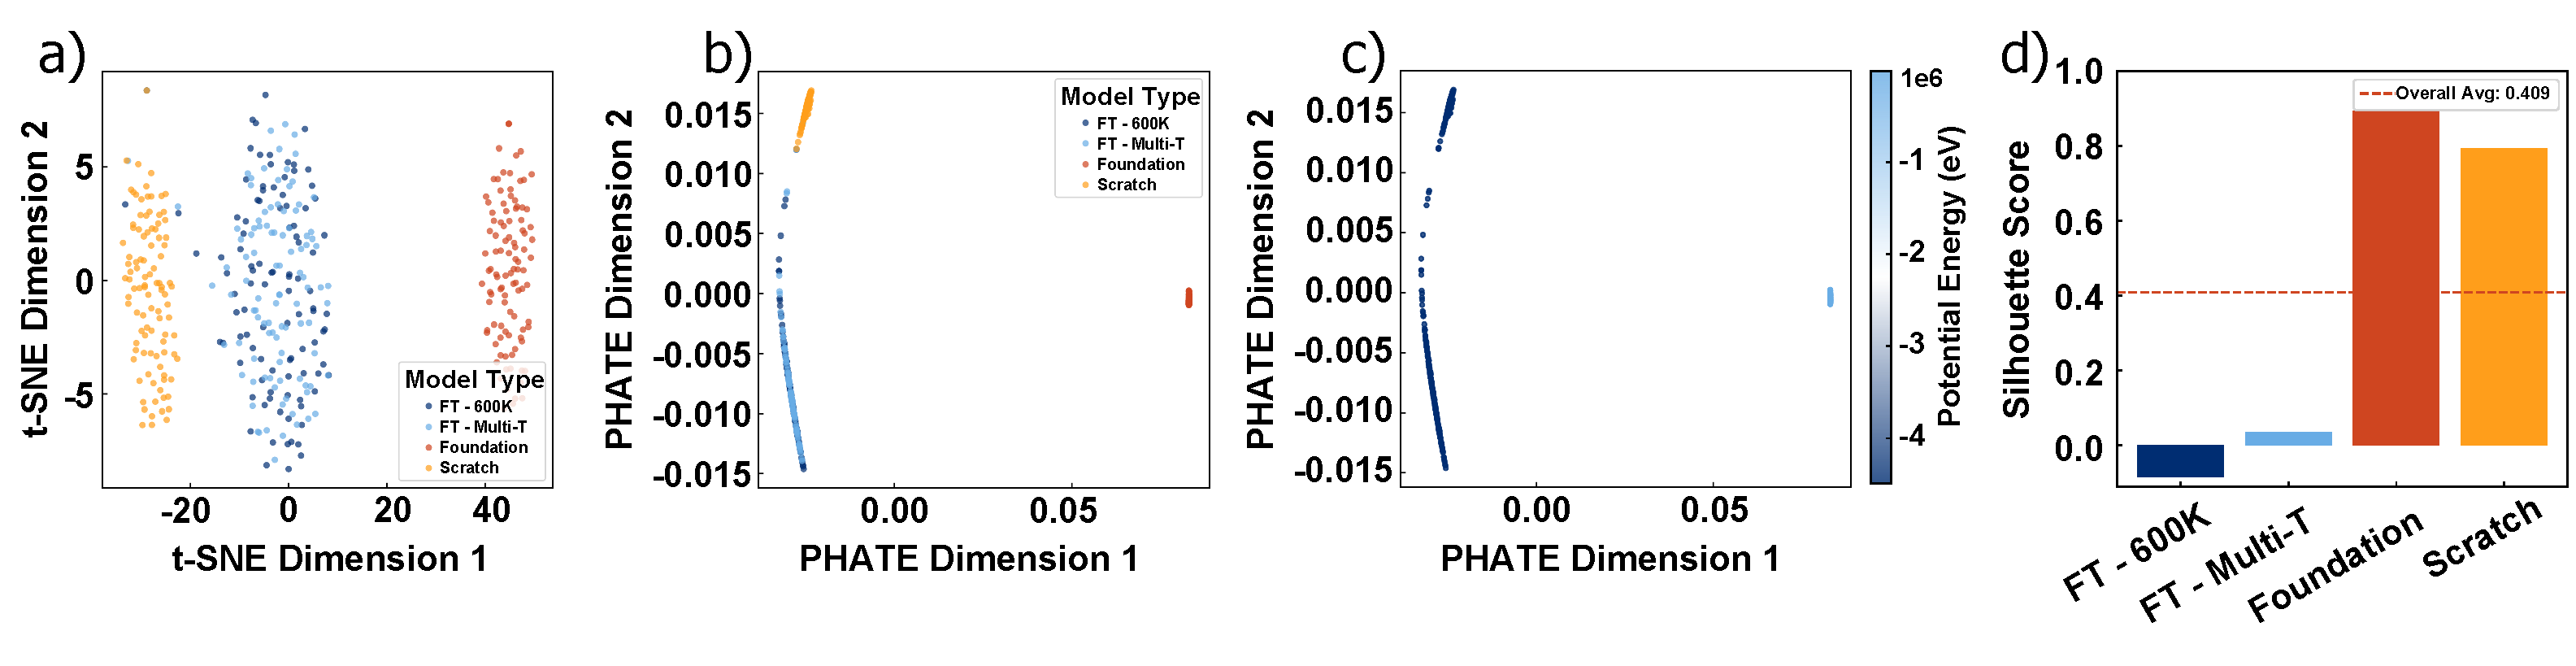
\includegraphics[width=\textwidth]{Fig/NeurIPS2025-AI4MAT-figure6-phate.pdf}
    \centering
    \caption{\textbf{Representation Analysis Reveals How Fine-Tuning Aligns a Physical Manifold to Enable Generalization.} Projections of atomic environment descriptors from 600~K MD trajectories. 
    \textbf{(a)}~A $t$-SNE projection shows that Foundation (red) and Scratch (orange) models produce highly separated representations, while fine-tuned models (blue) are intermediate. 
    \textbf{(b)}~PHATE projection reveals the system's continuous dynamical manifold. Note the clear separation between the brittle scratch model representation and the regularized fine-tuned models along the vertical axis (PHATE 2). 
    \textbf{(c)}~The same PHATE embedding, colored by potential energy, confirms that the manifold's geometry corresponds to the physical energy landscape. The foundation model's large energy offset indicates its nature as an uncalibrated prior.
\reviewermap{REV-C11}{done-local}{Silhouette values are recomputed in original descriptor space; projected values are retained only as a baseline.}
    \textbf{(d)}~Silhouette scores quantify separability in the original descriptor space and in low-dimensional embeddings. The projected values are used as visualization diagnostics, while the original-space values provide the primary quantitative check on representational dissimilarity.}
    \label{fig:tsne-phate}
\end{figure}


%%%%%%%%%% new parts for SHAP %%%%%%%%%%%%%


\subsection{Dissecting Learned Representations with Feature-Level Interpretability}

While $t$-SNE and PHATE reveals that distinct training strategies produce separable latent representations, it does not explain the underlying physical principles each model has learned. To bridge this gap, we move from \textit{what} the models learn to \textit{why} their performance diverges. We employ a rigorous interpretability framework based on SHapley Additive exPlanations (SHAP)~\cite{lundberg_unified_2017} to quantify the feature-level basis for model accuracy.

\reviewermap{REV-A6/REV-C13}{partial}{SHAP explains surrogate error predictions, not MACE internals directly; current 5-fold CV R2 values are 0.9819, 0.8756, and 0.9730.}
Our methodology is designed to identify descriptors correlated with predictive error. For each MACE model, we first trained a Gradient-Boosting Regressor as a surrogate model to predict the MACE model's absolute energy error based on the local atomic environment of each structure. The input features to this surrogate are the physically-grounded Smooth Overlap of Atomic Positions (SOAP) descriptors.~\cite{bartok2012representing} This approach interprets a simpler surrogate of the error landscape, not the internal message-passing mechanism of MACE itself. The current 5-fold cross-validation $R^2$ values for the audited surrogates are 0.9819, 0.8756, and 0.9730 [PLACEHOLDER: final per-model surrogate table and code-release hash]. We then applied TreeSHAP to these surrogate models, assigning feature-importance values to SOAP descriptors that are most correlated with prediction failures or successes in the surrogate task.


Our analysis reveals a divergence in the feature-importance landscapes learned by each training strategy. A global overview of the top 50 most influential SOAP descriptors across all models (Fig.~\ref{fig:shap}b) shows that the fine-tuned multi-temperature (FT–Multi-T) model develops a sparse, physically coherent representation, whereas the scratch-trained model distributes importance diffusely across many weak, noisy features. This contrast is consistent with the supplementary error and stability assessment (Fig.~S4), where the FT–Multi-T model exhibits both lower prediction errors and a substantially narrower error distribution. The SHAP-based feature-stability analysis (Fig.~S4c) further distinguishes consensus features—those consistently identified as important across all models—from non-consensus features, where the models strongly disagree. The consensus set predominantly consists of chemically intuitive descriptors involving Cr–Sb and Cr–Cr interactions (\textit{e.g.}, \texttt{Cr-Sb\_n13\_l0}, \texttt{Cr-Cr\_n22\_l0}), reflecting the core structural motifs governing local bonding stability in the Cr-doped Sb$_2$Te$_3$ lattice. In contrast, the non-consensus features (\textit{e.g.,} \texttt{Cr-Cr\_n42\_l4}, \texttt{Cr-Te\_n33\_l0}) display large variability in importance across models and primarily correspond to higher-order radial–angular couplings in more weakly constrained Sb–Sb, Sb–Te, and Cr–Te coordination shells. 
% This disagreement maps directly onto the differences in model performance: the fine-tuned models suppress these unstable, non-consensus descriptors, whereas the scratch-trained model relies on them—revealing that its poor performance originates from assigning importance to features that do not consistently encode physically meaningful interactions.

This disparity is quantified in Fig.~\ref{fig:shap}a, which compares the feature-importance profiles of the best and worst models. In the corrected surrogate analysis, the FT--Multi-T model assigns the largest mean absolute SHAP value to \texttt{Cr-Sb\_n43\_l0}, while the strongest scratch-model contributions are dominated by Cr--Te descriptors. The FT--Multi-T feature is consistent with sensitivity to Cr--Sb local coordination in the doped lattice, but a direct physical assignment requires perturbation tests rather than SHAP rankings alone [PLACEHOLDER: Cr--Sb local-environment perturbation test]. Conversely, the scratch model's diffuse surrogate-importance landscape and heavier reliance on non-consensus descriptors reflect a less stable error predictor, consistent with its difficulty on transition-state energetics and NEB stability.

% A broader, physics-based categorization of the features (Fig.~\ref{fig:shap}c) reinforces this finding. The FT--Multi-T model consistently assigns the highest importance to features characterized by long-range and high angular complexity. In contrast, the scratch model distributes its attention more evenly and ineffectively, particularly across simpler short-range and spherical interactions. This demonstrates that the fine-tuning process does not merely adjust parameters; it fundamentally re-weights the model's attention, distilling knowledge from the pre-trained foundation model to prioritize physically dominant interactions. This interpretability framework provides a quantitative, feature-level explanation for the model's learned chemical intuition and offers a powerful diagnostic tool for optimizing MLFF training protocols for specialized chemical systems.

%%%


\begin{figure}[h!]
    \centering
    
\includegraphics[width=0.95\linewidth]{figures/fig6_shap_revised.pdf}
    \caption{\textbf{SHAP-based Dissection of Feature Importance in MACE Models.}
    \textbf{(a)}~Mean absolute SHAP values for the top 50 SOAP features, comparing the best-performing fine-tuned model (FT--Multi-T) and the worst-performing scratch-trained model. The corrected audit identifies \texttt{Cr-Sb\_n43\_l0} as the largest mean absolute SHAP feature in the FT--Multi-T surrogate.
    % \yi{explicitly say the difference between the orbital }
    \textbf{(b)}~Heatmap of feature importance for the top 50 SOAP features across all training strategies. The FT--Multi-T model displays a sparse importance landscape, concentrating on a few key features, while the scratch model's landscape is diffuse and inefficient.
    % \textbf{(c)}~Aggregated SHAP importance across six physically-meaningful SOAP feature categories. The fine-tuned models consistently prioritize features with long-range and high angular complexity, indicating a more sophisticated learned representation of the underlying chemical physics.
    }
    \label{fig:shap}
\end{figure}

\section{Conclusions}

We benchmarked specialist (from-scratch) and generalist (foundation-based) MLFFs for Cr-doped \ce{Sb2Te3} using non-equilibrium configuration probes as a framework for evaluating both interpolation and extrapolation behavior. Diffusion trajectories and structured pathways revealed that, although all models reproduce equilibrium structures, their predictions diverge markedly under kinetically relevant distortions. These non-equilibrium probes therefore expose limitations that remain hidden under equilibrium-only validation.

\reviewermap{REV-A4}{done-local}{Broader principles are now framed as case-study hypotheses requiring cross-system validation.}
Our findings support several broader hypotheses. Robust benchmarking should span both in-distribution and out-of-distribution tasks, as accuracy near equilibrium does not guarantee kinetic fidelity. Fine-tuning enhances targeted performance but can reduce global physical generality, emphasizing the need for carefully designed adaptation strategies. Latent-space analysis shows that different training paradigms can produce qualitatively distinct representations, helping to diagnose why models with similar traditional metrics may behave differently in downstream tasks. Notably, the deep-penetration paths remain the most stringent OOD regime in this benchmark and are being finalized through restarted QE NEB calculations before final numerical ranking.

\reviewermap{REV-A4}{done-local}{Conclusion should keep framework generality as future validation rather than a final claim.}
Together, these results indicate that ``more data'' is not necessarily sufficient; task-relevant, non-equilibrium sampling is often the decisive ingredient for meaningful improvement. Migration-inspired probes, coupled with latent-space diagnostics and auditable data provenance, provide a practical route to identify which additional configurations are needed and where models are likely to fail. In this case study, the framework reframes the specialist--generalist debate: the goal is not to choose \textit{between} model classes, but to exploit the complementary strengths they offer while validating them against the specific non-equilibrium tasks they are expected to perform.

\section*{Acknowledgments}

\begin{itemize}
  \item \textbf{Funding} \\
This work was supported by the United States Department of Defense-funded Center of Excellence for Advanced Electro-photonics with 2D materials—Morgan State University, under Grant No. W911NF2120213. The authors thank Drs. Frank Gardea and Owen Vail, the cooperative agreement managers of the Center, for their interest and constructive comments. They also thank Dr. Ramesh Budhani for his guidance on the project.
YC thanks Johns Hopkins University for their support in AY 24–25. Computational resource support was provided by the petascale Hopkins facility, Advanced Research Computing at Hopkins (ARCH) (rockfish.jhu.edu), supported by National Science Foundation award OAC 1920103. Partial funding for ARCH’s infrastructure was originally provided by the State of Maryland.

  \item \textbf{Conflict of interest/Competing interests} \\
  The authors declare that they have no known competing financial interests or personal relationships that could have appeared to influence the work reported in this paper.

  \item \textbf{Ethics approval and consent to participate} \\
  Not applicable. This study does not involve human participants or animal subjects.

  \item \textbf{Consent for publication} \\
  Not applicable.

  \item \textbf{Data availability} \\
  The supporting dataset, including training manifests, NEB path metadata, model-predicted barriers, and post-processing tables, will be released through MigrationBench on Hugging Face at \url{https://huggingface.co/datasets/alinacao2000/MigrationBench} [PLACEHOLDER: final dataset DOI or commit hash]. The manifest records the source trajectory, split assignment, random seed, model provenance, DFT/MLFF task type, convergence status, and checksum for each derived artifact.

  \item \textbf{Materials availability} \\
  Not applicable. This work is entirely computational and does not involve the synthesis or distribution of physical materials.

  \item \textbf{Code availability} \\
\reviewermap{REV-C13}{pending-local}{Code release must include the working SHAP pipeline and remove or populate prior empty stubs.}
  The scripts used for data processing, DFT/MD post-processing, and plotting (including Cr configuration trajectory generation and PDOS analysis) are available on GitHub \url{https://github.com/yicao-elina/MigrationBench.git}.

  \item \textbf{Author contribution} \\
    \textbf{Y. C.}: conceptualization, methodology, data curation, DFT and MD simulations, analysis, visualization, and manuscript-writing. \textbf{P. M.}: literature review, conceptualization, and manuscript- writing. \textbf{P. C.}: conceptualization, project administration, supervision, funding acquisition, and manuscript-writing.
\end{itemize}


\bibliography{sn-bibliography}
% \bibliographystyle{sn-nature}



% \newpage
% \appendix


\end{document}
